\section{PMAC:一种并行的 MAC}\label{sec:6-11}

迄今为止,我们所介绍的所有 MAC 构造,包括 ECBC,CMAC 和 NMAC,本质上都是串行性的。也就是说,在第 $i-1$ 个分组的计算完成之前,无论如何都无法计算第 $i$ 个分组。这就使得我们很难利用硬件的并行性或流水线来加速 MAC 的生成和认证。在本节中,我们将介绍一种非常适合并行架构的安全 MAC,称作 PMAC。更具体地,我们将介绍一种名为 $\rm PMAC_0$ 的算法,因为它更容易描述。

令 $F_1$ 是一个定义在 $(\mathcal{K}_1,\mathbb{Z}_p,\mathcal{Y})$ 上的 PRF,其中 $p$ 是一个素数,$\mathcal{Y}:=\{0,1\}^n$。令 $F_2$ 是一个定义在 $(\mathcal{K}_2,\mathcal{Y},\mathcal{Z})$ 上的 PRF。

下面,我们构建一个新的 PRF,称作 $\rm PMAC_0$,它将一个密钥和一条 $\mathbb{Z}^{\leq\ell}_p$ 上的消息作为输入,输出 $\mathcal{Z}$ 上的一个元素。一个 $\rm PMAC_0$ 的密钥由 $k\in\mathbb{Z}_p$,$k_1\in\mathcal{K}_2$ 和 $k_2\in\mathcal{K}_2$ 组成。$\rm PMAC_0$ 构造的工作原理如下:

\vspace{5pt}

\hspace*{5pt} 输入:$m=(a_1,\dots,a_v)\in\mathbb{Z}^v_p$,其中 $0\leq v\leq\ell$,以及\\
\hspace*{75pt} 密钥 $\vec{k}=(k,k_1,k_2)$,其中 $k\in\mathbb{Z}_p$,$k_1\in\mathcal{K}_1$,$k_2\in\mathcal{K}_2$\\
\hspace*{26pt} 输出:$\mathcal{Z}$ 中的一个标签

\vspace{5pt}

\hspace*{5pt} ${\rm PMAC}_0(\vec{k},m)$:\\
\hspace*{50pt} 令 $t\leftarrow 0^n\in\mathcal{Y}$,$mask\leftarrow 0\in\mathbb{Z}_p$\\
\hspace*{50pt} 对于 $i=1,\dots,v$:\\
\hspace*{75pt} 令 $mask\leftarrow mask+k$ \quad\quad // $mask=i\cdot k\in\mathbb{Z}_p$\\
\hspace*{75pt} 令 $r\leftarrow a_i+mask$ \quad\quad\quad\; // $r=a_i+i\cdot k\in\mathbb{Z}_p$\\
\hspace*{75pt} 令 $t\leftarrow t\oplus F_1(k_1,r)$\\
\hspace*{50pt} 输出 $F_2(k_2,t)$

\vspace{5pt}

\noindent
在评估 $F_1$ 之前,主循环将掩码 $k,2k,3k,\dots$ 加到每个消息分组上。在一个串行设备上,这需要在每轮迭代中进行两次模 $p$ 加法。而在并行设备上,每个处理器都可以独立计算 $a_i+i\cdot k$,然后将其应用到 $F_1$ 上,如图 \ref{fig:6-9} 所示。

$\rm PMAC_0$ 是一个安全的 PRF,因此对于长的消息来说,$\rm PMAC_0$ 可以作为一个安全的 MAC。根据下一章的定理 \ref{theo:7-7},我们很容易给出它的安全性证明。现在,我们先说明该定理,并将对它的证明留到 \ref{subsec:7-3-3} 小节。

\begin{figure}
  \centering
  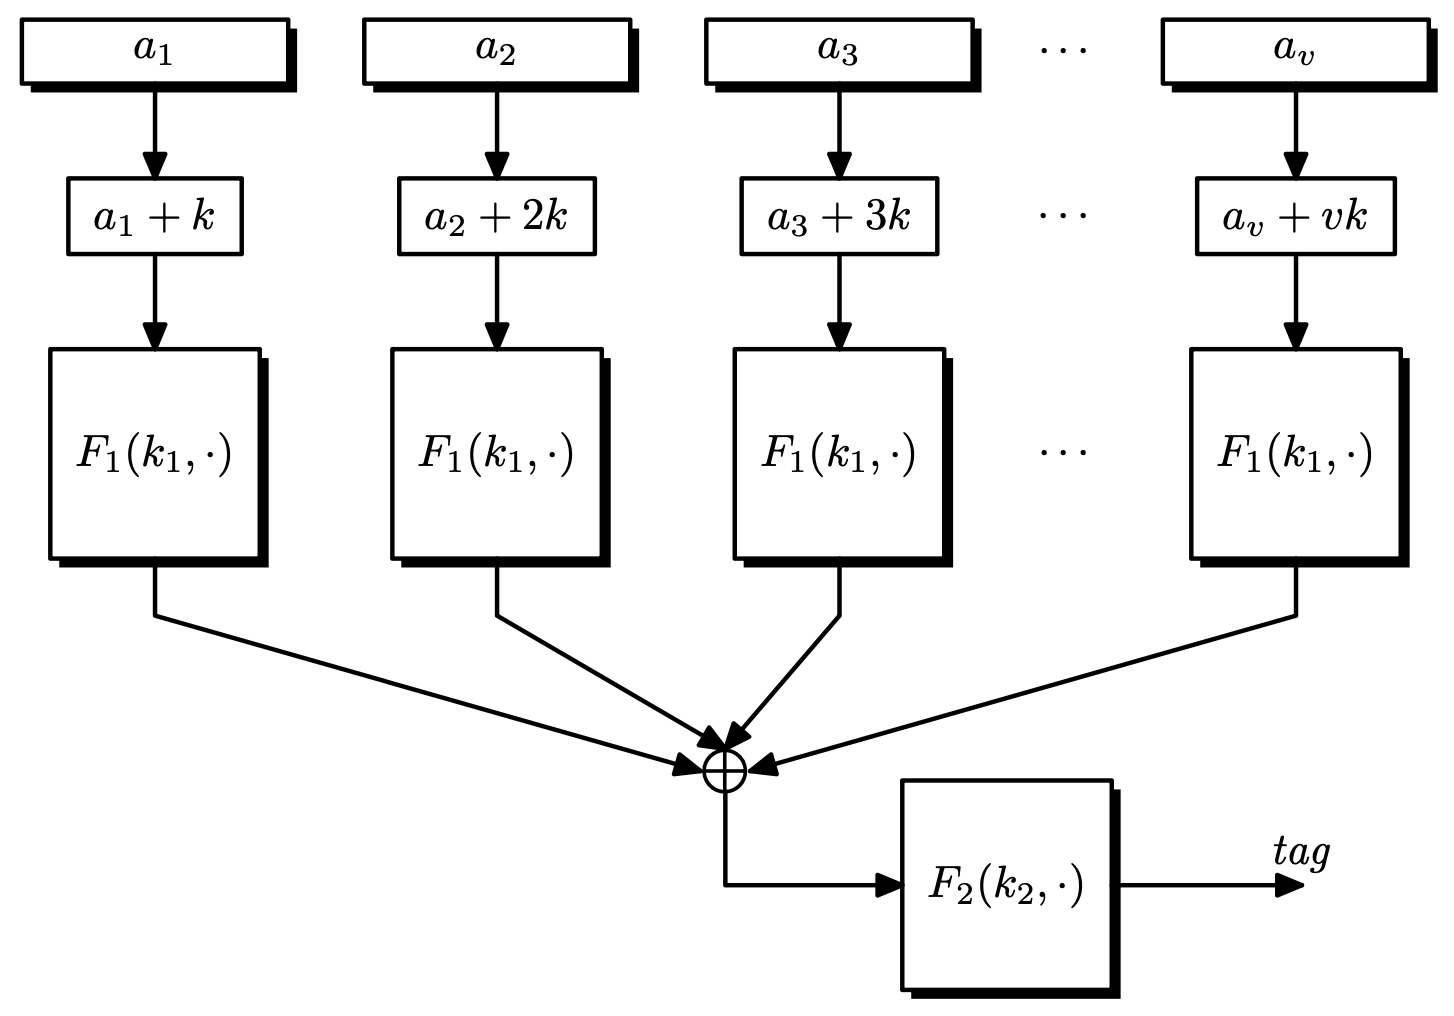
\includegraphics[width=0.6\linewidth]{figures/chapter6/fig9.png}
  \caption{$\rm PMAC_0$ 构造}
  \label{fig:6-9}
\end{figure}

\begin{theorem}\label{theo:6-11}
如果 $F_1$ 和 $F_2$ 都是安全的 PRF,且 $|\mathcal{Y}|$ 和素数 $p$ 都是超多项式的,那么 $\rm PMAC_0$ 对于任何多项式约束的 $\ell$ 都是安全的 PRF。
\begin{quote}
特别地,对于每个按照攻击游戏 \ref{game:4-2} 攻击 $\rm PMAC_0$ 的 PRF 对手 $\mathcal{A}$,假设它最多能够向其挑战者发起 $Q$ 次查询,则必然存在两个 PRF 对手 $\mathcal{B}_1$ 和 $\mathcal{B}_2$,其中 $\mathcal{B}_1$ 和 $\mathcal{B}_2$ 都是围绕 $\mathcal{A}$ 的基本包装器,满足:
\end{quote}
\begin{equation}\label{eq:6-28}
{\rm PRF}\mathsf{adv}[\mathcal{A}, {\rm PMAC_0}]\leq{\rm PRF}\mathsf{adv}[\mathcal{B}_1,F_1]+{\rm PRF}\mathsf{adv}[\mathcal{B}_2,F_2]+\frac{Q^2}{2|\mathcal{Y}|}+\frac{Q^2\ell^2}{2p}
\end{equation}
\end{theorem}

当使用 $\rm PMAC_0$ 时,我们要把输入消息切分成多个分组,其中的每个分组都是 $\mathbb{Z}_p$ 中的元素。在实践中,这是很不方便的。相对地,将每条消息切分成 $\{0,1\}^n$ 中的 $n$ 比特序列就要容易得多。接下来介绍的一个更好的并行 MAC 构造,正是通过使用有限域 ${\rm GF}(2^n)$ 代替 $\mathbb{Z}_p$ 实现的。这是一个很好的例子,能够说明为什么有限域 ${\rm GF}(2^n)$ 在密码学中如此重要。出于安全考虑,我们经常需要将计算定义在某个域上,但是像 $\mathbb{Z}_p$ 这样的素阶有限域在实践中总是不太方便。${\rm GF}(2^n)$ 相对来说就要好很多,它上面的算术运算更快,还能很自然地让我们对 $n$ 比特序列进行操作。

\begin{snote}[比 $\rm PMAC_0$ 更好的 PMAC。]
尽管 $\rm PMAC_0$ 非常适合用在并行硬件上,但它仍然有改进空间。事实上,还有一些比 $\rm PMAC_0$  更优秀的实现,包括 PMAC 和 XECB,它们都是可并行的。具体地,PMAC 相对 $\rm PMAC_0$ 来说有如下的改进:
\begin{itemize}
	\item PMAC 使用有限域 ${\rm GF}(2^n)$ 上的算术运算,而不是 $\mathbb{Z}_p$。${\rm GF}(2^n)$ 中的元素可以表示为 $n$ 比特长的序列,域上的加法就是按位异或。正因如此,PMAC 实际上只是使用了 $F_1=F_2=F$,其中 $F$ 是定义在 $(\mathcal{K},\mathcal{Y},\mathcal{Y})$ 上的一个 PRF。PMAC 的输入空间由 $\mathcal{Y}=\{0,1\}^n$ 中的元素序列组成,而不是 $\mathbb{Z}_p$ 中的元素。
	\item PMAC 的第 $i$ 分组的掩码被定义为 $\gamma_i\cdot k$,其中 $\gamma_1,\gamma_2,\dots$ 是 ${\rm GF}(2^n)$ 中的固定常数。乘法也定义在 ${\rm GF}(2^n)$ 上。$\gamma_i$ 是经过特别选取的,为的是保证从 $\gamma_i\cdot k$ 计算 $\gamma_{i+1}\cdot k$ 成本很低。
	\item PMAC 的密钥 $k$ 是由 $k\leftarrow F(k_1,0^n)$ 派生而来的,并且令 $k_2\leftarrow k_1$。因此,PMAC 使用的密匙比 $\rm PMAC_0$ 的更短。
	\item PMAC 使用一个技巧来保存 $F$ 的一个应用。
	\item PMAC 使用 CMAC $rpf$ 的一个变体来提供按位 PRF。
\end{itemize}
结果就是,PMAC 在串行设备上与 ECBC 和 NMAC 的效率相近,但在并行或流水线设备上有更好的性能。PMAC 在本章所介绍的所有 PRF 中是最优秀的,它在各种计算机结构上都能很好地工作,对长消息和短消息都很有效。
\end{snote}

\begin{snote}[$\rm PMAC_0$ 是增量的。]
假设 Bob 为某一条长消息 $m$ 计算了标签 $t$,一段时间后他改变了 $m$ 中的一个分组,想要重新计算这条新消息 $m'$ 的标签。当使用 CBC-MAC 时,现在的标签 $t$ 对于新的计算是毫无用处的——Bob 必须从头开始计算 $m'$ 的新标签。但使用 $\rm PMAC_0$ 时,情况就会有很大的改观。假设用于构造 $\rm PMAC_0$ 的 PRF $F_2$ 是一个分组密码,比如 AES,令 $D$ 为该分组密码的解密算法。令 $m'$ 是将 $m$ 的第 $i$ 个分组从 $a_i$ 修改为 $a_i'$ 后得到的新消息。那么,我们很容易由 $m$ 的标签 $t:={\rm PMAC_0}(k,m)$ 推导出 $m'$ 的新标签 $t':={\rm PMAC_0}(k,m')$,方法如下:

\vspace{5pt}

\hspace*{5pt} 令 $t_1\leftarrow D(k_2,t)$\\
\hspace*{26pt} 令 $t_2\leftarrow t_1\oplus F_1(k_1,\;a_i+i\cdot k)\oplus F_1(k_1,\;a_i'+i\cdot k)$\\
\hspace*{26pt} 令 $t'\leftarrow F_2(k_2,t_2)$

\vspace{5pt}

\noindent
因此,给定某个长消息 $m$ 的标签(以及 MAC 的密钥),我们很容易推导出对 $m$ 进行局部修改后的新标签。具有这种性质的 MAC 被称作是\textbf{增量的(incremental)}。我们上面标明,使用分组密码实现的 $\rm PMAC_0$ 是增量的。
\end{snote}